%\documentclass[a4paper,10pt]{article}
\documentclass[12pt]{article}
\usepackage{graphicx}
\usepackage{amssymb}
\usepackage{amsmath}
\usepackage{longtable}
\usepackage{wrapfig}
%\usepackage{color}
%\usepackage{amsthm}
\usepackage[utf8]{inputenc}
\usepackage[T1]{fontenc}
\usepackage{lmodern}
\usepackage{listings}
\usepackage[usenames,dvipsnames]{color}
\usepackage{fancyhdr}
\usepackage{fullpage}
%\usepackage[top=tlength, bottom=blength, left=llength, right=rlength]{geometry}
%\usepackage{geometry}
%\usepackage[a4paper]{geometry}
\definecolor{MyDarkGreen}{rgb}{0.0,0.4,0.0}
%\usepackage[pdftex]{graphicx}
%\usepackage{mathtools}
\usepackage{listings}
\lstset{language=R}
%===========================================================================================
% Numbering Equations
%\numberwithin{equation}{section} %sets equation numbers <chapter>.<section>.<index>
\numberwithin{equation}{subsection} %sets equation numbers <chapter>.<section>.<subsection>.<index>
%\numberwithin{equation}{subsubsection} %sets equation numbers <chapter>.<section>.<subsection>.<subsubsection>.<index>


%===================================================================================================================
% Basic Commands for Page settings,Chapters, Appendices, Sections, etc..
%====================================================================================================================
%\setlength{\oddsidemargin}{.5in} \setlength{\topmargin}{0in}
%\setlength{\headheight}{.2in} \setlength{\headsep}{.2in}
%\setlength{\textwidth = 6.0in} \setlength{\textheight = 8.3in}

\setlength{\oddsidemargin}{0.6in} \setlength{\topmargin}{-0.3in} %adjust side margins and top margins
\setlength{\headheight}{.2in} \setlength{\headsep}{.2in}
\setlength{\textwidth = 6.0in} \setlength{\textheight = 8.3in}



\def\thebiblio#1{\list
{[\arabic{enumi}]}{\settowidth\labelwidth{[#1]}\leftmargin\labelwidth
\advance\leftmargin\labelsep
\usecounter{enumi}}
\def\newblock{\hskip .11em plus .33em minus .07em}
\sloppy\clubpenalty4000\widowpenalty4000
\sfcode`\.=1000\relax}
\let\endthebiblio=\endlist

\newcommand{\sect}[1]{% Basic settings for general chapters
\cleardoublepage
\clearpage
\newpage
\begin{center}
\addtocounter{section} {1}
\setcounter{subsection} {0}
\section* {\normalsize \bf{CHAPTER \thesection \\ #1}}
\addcontentsline{toc}{section}{CHAPTER
\protect\numberline{\thesection : } #1\dotfill}
\end{center}
\thispagestyle{myheadings} }

\newcommand{\appen}[1]{% Basic settings for appendix chapters
\cleardoublepage
\clearpage
\newpage
\begin{center}
\addtocounter{section} {1}
\renewcommand{\thesection}{\Alph{section}}
\setcounter{subsection} {0}
\setcounter{table}{0}
\section* {\normalsize \bf{APPENDIX \thesection \\ #1}}
\addcontentsline{toc}{section}{APPENDIX
\protect\numberline{\thesection : } #1\dotfill}
\end{center}
\renewcommand{\thesubsection}{\Alph{section}.\arabic{subsection}}
\renewcommand{\thesubsubsection}{\Alph{section}.\arabic{subsection}.\arabic{subsubsection}}
\renewcommand{\theequation}{\Alph{section}.\arabic{equation}}
\renewcommand{\thetable}{\Alph{section}.\arabic{table}}

\thispagestyle{myheadings} }

%===================================================================================================================
% Basic Commands for Theorem, Lemma,Proposition,etc.....

\renewcommand{\baselinestretch}{2}
\renewcommand{\arraystretch}{.5}
\newcommand{\qed}{\hfill$\Box$}
\newtheorem{fact}{Theorem}[section]
\newtheorem{claim}{Claim}
\newtheorem{theorem}[fact]{Theorem}
\newtheorem{word}[fact]{Definition}
\newtheorem{prop}[fact]{Proposition}
\newtheorem{ob}[fact]{Observation}
\newtheorem{Corollary}[fact]{Corollary}
\newtheorem{corollary}[fact]{Corollary}
\newtheorem{lemma}[fact]{Lemma}
\newtheorem{Guess}[fact]{Conjecture}
\newtheorem{conj}[fact]{Conjecture}
\def\theotheorem{A\arabic{theorem}}
\newtheorem{mydef}{Definition}
%\newtheorem{theorem}{Theorem}[section]
%\newtheorem{lemma}[theorem]{Lemma}
%\newtheorem{proposition}[theorem]{Proposition}
\newtheorem{thm}{Theorem}
\newtheorem{lem}{Lemma}[thm]
%\newtheorem{corollary}[theorem]{Corollary}
%\newtheorem{cor}[theorem]{Corollary}
\newenvironment{proof}[1][Proof]{\begin{trivlist}
\item[\hskip \labelsep {\bfseries #1}]}{\end{trivlist}}
\newenvironment{definition}[1][Definition]{\begin{trivlist}
\item[\hskip \labelsep {\bfseries #1}]}{\end{trivlist}}
\newenvironment{example}[1][Example]{\begin{trivlist}
\item[\hskip \labelsep {\bfseries #1}]}{\end{trivlist}}
\newenvironment{remark}[1][Remark]{\begin{trivlist}
\item[\hskip \labelsep {\bfseries #1}]}{\end{trivlist}}
%================================================================================
%%%%%%%%%%%commands for problem
%================================================================================
\makeatletter
\newenvironment{problem}{\@startsection
       {section}
       {1}
       {-.2em}
       {-3.5ex plus -1ex minus -.2ex}
       {2.3ex plus .2ex}
       {\pagebreak[3]%forces pagebreak when space is small; use \eject for better results
       \large\bf\noindent{Problem }
       }
       }
       {%\vspace{1ex}\begin{center} \rule{0.3\linewidth}{.3pt}\end{center}}
       \begin{center}\large\bf \ldots\ldots\ldots\end{center}}
\makeatother


%
%Fancy-header package to modify header/page numbering
\pagestyle{fancy}
%\addtolength{\headwidth}{\marginparsep} %these change header-rule width
%\addtolength{\headwidth}{\marginparwidth}
\lhead{Problem \thesection} \chead{} \rhead{\thepage}
\lfoot{\small\scshape course name} \cfoot{} \rfoot{\footnotesize
PS\#}
\renewcommand{\headrulewidth}{0.3pt}
\renewcommand{\footrulewidth}{.3pt}
%\setlength\voffset{-0.25in} \setlength\textheight{648pt} \maketitle
%\maketitle
 %\thispagestyle{empty}



%===========================================================================
% commands for displaying codes in appendix
%============================================================================
\lstloadlanguages{R}%
\lstset{language=R,                        % Use R
        %frame=single,                           % Single frame around code
        basicstyle=\small\ttfamily,             % Use small true type font
        keywordstyle=[1]\color{Blue}\bf,        % MATLAB functions bold and blue
        keywordstyle=[2]\color{Purple},         % MATLAB function arguments purple
        keywordstyle=[3]\color{Blue}\underbar,  % User functions underlined and blue
        identifierstyle=,                       % Nothing special about identifiers
                                                % Comments small dark green courier
        commentstyle=\usefont{T1}{pcr}{m}{sl}\color{MyDarkGreen}\small,
        stringstyle=\color{Purple},             % Strings are purple
        showstringspaces=false,                 % Don't put marks in string spaces
        tabsize=5,                              % 5 spaces per tab
        %
        %%% Put standard MATLAB functions not included in the default
        %%% language here
        morekeywords={xlim,ylim,var,alpha,factorial,poissrnd,normpdf,normcdf},
        %
        %%% Put MATLAB function parameters here
        morekeywords=[2]{on, off, interp},
        %
        %%% Put user defined functions here
        morekeywords=[3]{FindESS, homework_example},
        %
        morecomment=[l][\color{Blue}]{...},     % Line continuation (...) like blue comment
        numbers=left,                           % Line numbers on left
        firstnumber=1,                          % Line numbers start with line 1
        numberstyle=\tiny\color{Blue},          % Line numbers are blue
        stepnumber=5                            % Line numbers go in steps of 5
        }

% Includes a MATLAB script.
% The first parameter is the label, which also is the name of the script
%   without the .m.
% The second parameter is the optional caption.
\newcommand{\matlabscript}[2]
  {\begin{itemize}\item[]\lstinputlisting[caption=#2,label=#1]{#1.r}\end{itemize}}





\begin{document}
\pagestyle{empty}
\pagenumbering{roman}

%================================================ Approval Page ===================================================


\newpage
%================================================ Title Page ======================================================
\begin{center}
\thispagestyle{empty} % takes out page numbering
  {ADVANCED MACROECONOMICS MID SEMESTER TEST\\ [.07in]} \rm
\rule{1.25in}{.01in}\\[.0 in]
\today
\vspace{.6in}



\vspace{.6in}

\vspace{.6in}

by  \\ [.06in]
{Nana  Akwasi Abayie Boateng} \\[.06in]
\end{center}
\author{Nana Akwasi Abayie Boateng\footnotemark[1]}












\def\R{\mathbb{R}}
\def\N{\mathbb{N}}
\def\Z{\mathbb{Z}}
\def\Q{\mathbb{Q}}
\def\la{\langle}
\def\ra{\rangle}

\def\dist{{\rm dist}}
\def\X{{\bf X}}
\def\C{{\bf C}}
\def\D{{\bf D}}
\def\I{{\bf I}}
\def\J{{\bf J}}
\def\x{{\bf x}}
\def\y{{\bf y}}
\def\z{{\bf z}}
\def\W{{\bf W}}
\def\g{{\bf g}}
\def\e{{\bf e}}
\def\b{{\bf b}}
\def\u{{\bf u}}
\def\Beta{{\bf \beta}}
\def\pen{{\rm pen}}
\def\argmin{{\rm argmin}}
\def\diag{{\rm diag}}
\def\sgn{{\rm sgn}}
\def\supp{{\rm\rm supp}}


\vspace*{1cm}
%============================================= Appendix Separation Page  ===============================================
\newcommand{\Appendixpage}{
    \setcounter{section}{0}
    \renewcommand{\baselinestretch}{1}\small\normalsize
    \thispagestyle{myheadings}
    \addcontentsline{toc}{section}{APPENDICES\dotfill}
    \mbox{}
    \vfil
    \begin{center}%
    APPENDICES
    \vfil
    \end{center}%
    \renewcommand{\baselinestretch}{1.66} \small\normalsize%
    \cleardoublepage
  }

%================================================ Chapter 1 ==============================================================

\newpage
\section{Question 1}


%$$H(E,R,p)=U(e_{1}+e_{2})-\alpha(k_{1}e_{1}+k_{2}e_{2})-p(e_{1}}$$
%$U(e_{1}+e_{2})-\alpha(k_{1}e_{1}+k_{2}e_{2})-p(e_{1}}$
\begin{equation}
u=u(e_{1}+e_{2})-\alpha(k_{1}e_{1}+k_{2}e_{2})-pe_{1}
 \end{equation}

\begin{equation}
\frac{\partial H}{\partial e_{1}}=U^{\prime}(e_{1}+e_{2})-\alpha k_{1}-p\geq 0
 \end{equation}

FOCS:
\begin{equation}
\frac{\partial H}{\partial e_{2}}=U^{\prime}(e_{1}+e_{2})-\alpha k_{2}\geq 0
 \end{equation}

\begin{equation}
\lim_{t \to \infty}e^{-\rho t}p(t)R(t)= 0
 \end{equation}

\begin{equation}
\frac{\partial H}{\partial R}=\rho p-\dot{p}= 0
 \end{equation}


\begin{equation}
\frac{\dot{p}}{p}=\rho= 0
 \end{equation}
\begin{equation}
\frac{d{p}}{p}=\rho dt= 0
 \end{equation}

\section{Question 2}
\begin{equation}
\frac{d{p}}{p}=\rho dt= 0
 \end{equation}
\begin{equation}
\int \frac{d{p}}{p}=\int \rho dt= 0
 \end{equation}

\begin{equation}
\ln (p)=\rho t+c
 \end{equation}
\begin{equation}
p(t)=A\exp({\rho t})
 \end{equation}
$at t= 0,A=p(0)$
\begin{equation}
p(t)=p(0)\exp({\rho t})
 \end{equation}


\section{Question 3}
using alternative technogy, the marginal utility of alternative technology\\

$ u^{\prime}(e_{1}+e_{2})= \alpha k_{2} $\\

$(e_{1}+e_{2})=u^{\prime-1}(\alpha k_{2})$\\

$\bar{e}=u^{\prime-1}(\alpha k_{2})$\\



\section{Question 4}
using extractive technogy, the marginal utility of alternative technology\\

$U^{\prime}(e_{1}+e_{2})-\alpha k_{1}-p= 0$\\

$U^{\prime}(e_{1}+e_{2})=\alpha k_{1}+p$\\

$p(t)=p(0)\exp(\rho t)$\\

$U^{\prime}(e_{1}+e_{2})(t_{1})=\alpha k_{1}+p(t_{1})$\\

$U^{\prime}(e_{1}+e_{2})(t_{2})=\alpha k_{1}+p(t_{2})$\\

$U^{\prime}(e_{1}+e_{2})(t_{1})=\alpha k_{1}+p(0)\exp(\rho t_{1})$\\

$U^{\prime}(e_{1}+e_{2})(t_{2})=\alpha k_{1}+p(0)\exp(\rho t_{2})$\\
U is strictly concave,which implies its derivative is decreasing on $[t_{1},t_{2}]$\\
$U^{\prime}(e_{1}+e_{2})(t_{1}) >U^{\prime}(e_{1}+e_{2})(t_{2})$

\begin{equation}
U^{\prime}(e_{1}+e_{2})(t)=\alpha k_{1}+p(0)\exp(\rho t)
 \end{equation}

\section{Question 5}
On the interval $[t_{1},t_{2}] $ where $t_{1}<t_{2}$.The marginal utility at $t_{1}$ is greater that at $t_{1}$.The technology with the higher marginal utility will be chosen at each time period.
$U^{\prime}(e_{1}+e_{2})(t_{1}) >U^{\prime}(e_{1}+e_{2})(t_{2})$


\section{Question 6}
$U^{\prime}(e_{1}+e_{2})-\alpha k_{1}-p= U^{\prime}(e_{1}+e_{2})-\alpha k_{2}$\\

$p(T)=\alpha k_{1}-\alpha k_{2}$\\
$p(T)=p(0)\exp(\rho T)$

$p(0)\exp(\rho T)=\alpha k_{1}-\alpha k_{2}$\\



\section{Question 7}
$U^{\prime}(e_{1}+e_{2})-\alpha k_{1}-p= U^{\prime}(e_{1}+e_{2})-\alpha k_{2}$\\

$p(T)=\alpha k_{1}-\alpha k_{2}$\\
$p(T)=p(0)\exp(\rho T)$

$p(0)\exp(\rho T)=\alpha k_{1}-\alpha k_{2}$\\

$p(0)=\frac{\alpha k_{1}-\alpha k_{2}}{\exp(\rho T)}$

\section{Question 8}
$U^{\prime}(e_{1}+e_{2})-\alpha k_{1}-p=0$\\

$U^{\prime}(e_{1}+e_{2})=\alpha k_{1}+p$\\

$U^{\prime}(e_{1}+e_{2})=\alpha k_{1}+p(0)\exp(\rho t)$\\

$\int _{t}^{T}\frac{dp}{p}=\int_{t}^{T} \rho dt$

$\ln(p(T))-\ln(p(t))=\rho(T-t)$\\

$\ln \left( \frac{p(T)}{p(t)} \right)= \rho(T-t)$\\

$\frac{p(T)}{p(t)}=exp(\rho(T-t))$\\

$p(t)=p(T)exp(\rho(T-t))$\\

$U^{\prime}(e_{1}+e_{2})=\alpha k_{1}+p(T)exp(\rho(T-t))$\\

$e_{1}+e_{2}=U^{\prime-1}(\alpha k_{1}+p(T)exp(\rho(T-t)))$\\

$e_{1}=e_{2}+U^{\prime-1}(\alpha k_{1}+p(T)exp(\rho(T-t)))$\\

\section{Question 9}

\begin{equation}
\dot{R}=-e_{1}
\end{equation}


\begin{equation}
\frac{d R}{dt}=-e_{1}
\end{equation}


\begin{equation}
{d R}=-e_{1}dt
\end{equation}


\begin{equation}
\int_{0}^{T}{d R}=-\int_{0}^{T}e_{1}dt
\end{equation}

\begin{equation}
\int_{0}^{T}{d R}=-\int_{0}^{T}\left[ e_{2}+U^{\prime-1}(\alpha k_{1}+p(T)exp(\rho(T-t))) \right]dt
\end{equation}



\section{Question 10}
\vspace{100mm}
\newpage

\section{Question 11}
The graphs below were plotted by fixing these parameters.\\
$p(0)=5, \rho=0.2,t=[0,100]$
\begin{figure}[ht!]
\centering
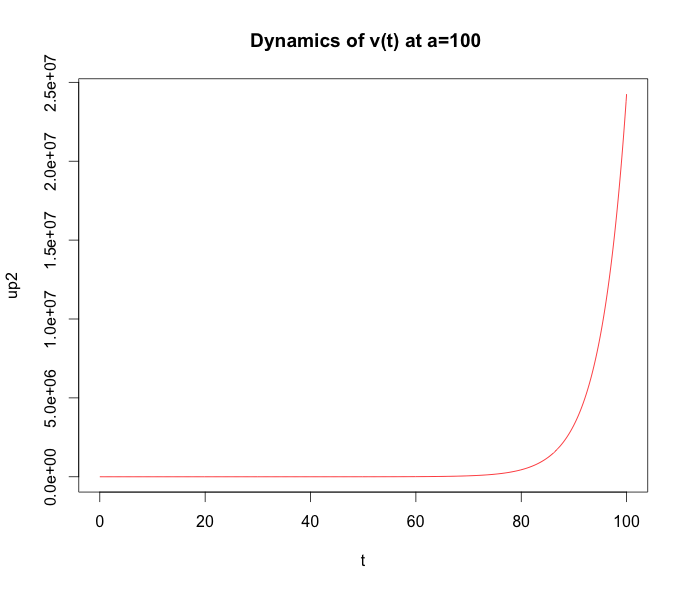
\includegraphics[width=170mm,height=170mm]{11.png}
\caption{ Dynamics of V(t) at a=100 k\label{overflow}}
\end{figure}
\newpage
\section{Question 12}
Increasing $\alpha$ decreases the marginal utility whereas decreasing it increases the marginal utility.\\
increase in $\alpha$ decreases $v(t)$,the marginal price of energy at $t$ in terms of the general good
\begin{figure}[ht!]
\centering
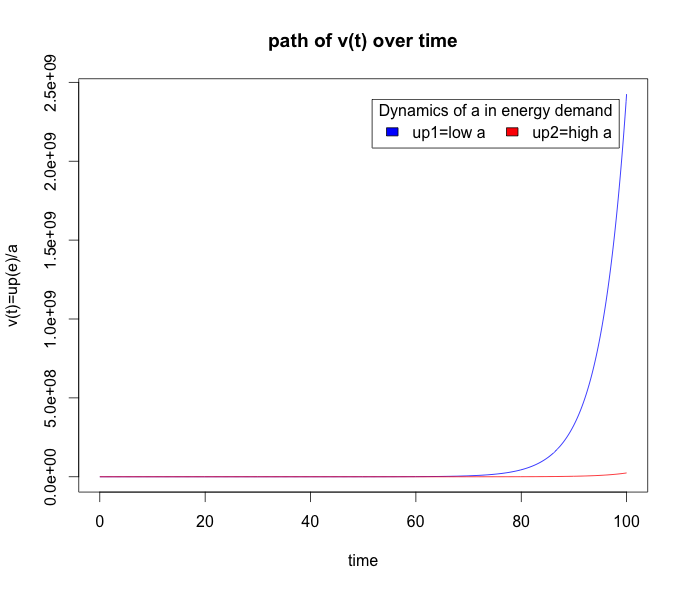
\includegraphics[width=170mm,height=170mm]{final.png}
\caption{Dynamics of V(t) at up2 with a=100 and up1 with a=1\label{overflow}}
\end{figure}
\newpage
\begin{figure}[ht!]
\centering
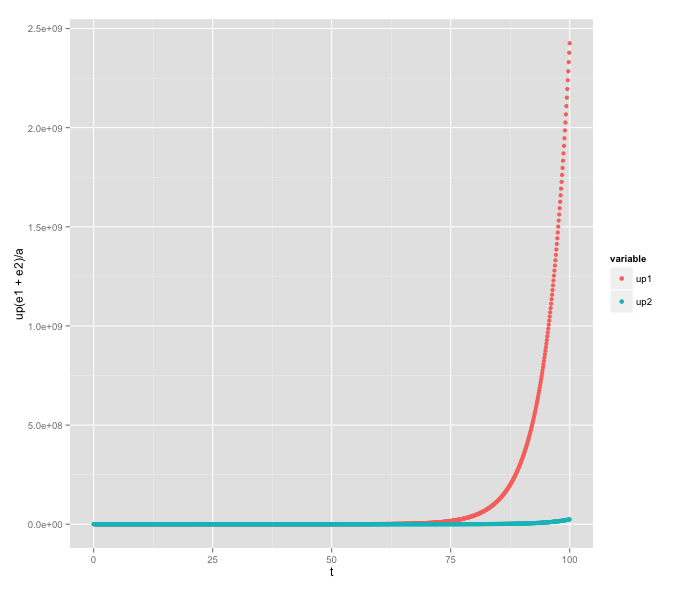
\includegraphics[width=170mm,height=170mm]{final2.png}
\caption{Dynamics of V(t) at  up2 with a=100 and up1 with a=1\label{overflow}}
\end{figure}
newpage
\begin{figure}[ht!]
\centering
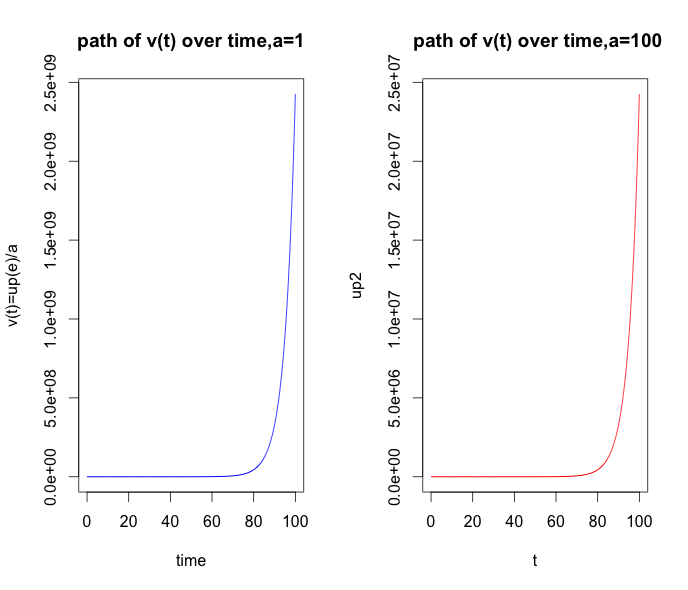
\includegraphics[width=170mm,height=170mm]{11b.png}
\caption{Dynamics of V(t) at  up2 with a=100 and up1 with a=1\label{overflow}}
\end{figure}
%=================================================BIBLIOGRAPHY==============================================================
%\newpage
%\begin{center}
%{\bf BIBLIOGRAPHY}
%\end{center}
%\addcontentsline{toc}{section}{\rm BIBLIOGRAPHY \dotfill}
%\begin{thebiblio}{99}
%---------------------------------------------------------------------------------------------------------------------------




%\bibitem{PSJ}
%Paul Wilmott,Sam Howson,Jeff Dewynne  \emph{The Mathematics of
%Financial Derivatives}. A Student Introduction, Cambridge university
%press.

%\bibitem{CF}
%Omur Ogur \emph{An Introduction to Computational Finance}.Imperial
%College press




%\bibitem{GEF}
%G.E. Fasshauer,\emph{Meshfree Methods}.Handbook of Theoretical and
%Computational Nanotechnology,M.Rieth and W.Schommers(eds.).American
%Scientific Publishers .(2006)
%\end{thebiblio}
\newpage
%=================================Appendix separation page ===========================================================
%\Appendixpage
%---------------------------------------------------------------------------------------------------------------------

%%================================================= Appendix A =========================================================
%\appen{\uppercase{ Sample Appendix}}\label{app1}
%%-------------------------------------------------------------------------------------------------------------------






%=========================Appendix ===================================================================================
%\appen{\uppercase{Computer Programming Codes}}\label{app2}
%----------------------------------------------------------------------------------------------------------------------

\subsection{R  Programming Codes}

\lstinputlisting{uprime.R}
%\subsubsection{Theta method codes}
%\lstinputlisting{RBasis3GaussianG.m}
%\lstinputlisting{RBasis3GaussianMQ.m}
%\lstinputlisting{RBasis3GaussianIMQ.m}
%\lstinputlisting{tridiagonal.m}




\end{document}
